\section{Structure du projet}
\subsection{Modèle Vue/Controlleur}
Pour l'apparence visuel du site nous avons adopté le modèle vue/controlleur. \\
Cela s'avère particulièrement utile pour l'affichage du header qui permet à l'utilisateur d'accéder à toutes les fonctionnalités du site, et ce quelque soit la page sur laquelle il se trouve actuellement.\\
Chaque page du site inclus donc la vue de ce header en entête, puis une vue de la page en question.
Par exemple la page login.php inclus la vue header.php ainsi que la vue de login.php (une autre page qui n'est pas dans public).\\
L'affichage des images de profil est aussi gérée par des vues et plus précisément par des fonctions php qui permettent d'afficher une image et de décider de ses dimensions ainsi que de sa forme en retournant une balise avec du CSS.\\
On retrouve dans le dossier \texttt{/public/Forms} les fichiers php qui s'occupe de la manipulation de la base de donnée côté serveur, avec par exemple \texttt{login.php} ou \texttt{addKara.php}.\newline
Les interfaces User, Lector, Playlist, et Kara se trouvent respectivement dans leur dossier respectifs dans le \texttt{/src}.


\subsection{Apparence visuelle}
Pour assurer qu'aucun style directement implémenté dans le html ne se fasse écraser par la feuille de style, l'utilisation de classe à été privilégié pour mieux contrôler les balises sur lesquelles le style s'applique. Une feuille de style, style.css, est commune à toutes les pages (car présente dans le \texttt{src/View/Layout/head.php} que l'on inclus systématiquement). Il est cependant possible d'intégrer d'autres feuilles de style pour des pages spécifiques.

\subsection{la base de donnée}
On rajoute plusieurs tables à la base de données pour pouvoir gérer les cosmétiques de chaque utilisateur, leur playlist, la queue et la liste des lecteur du côté de lektor. Voici le diagramme UML de la base de donnée du site:
\newline
\begin{figure}[h!]
\centering
\hspace*{-1.2in}
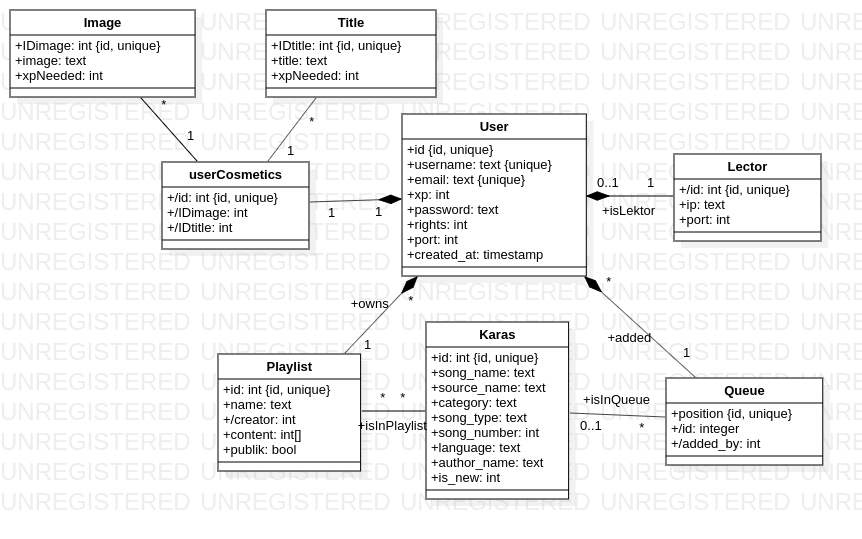
\includegraphics[scale=0.6]{UML.png}
\caption{diagramme UML de la base}
\label{fig:diagramme UML}
\end{figure}
\newpage
